%\documentclass[a4paper]{article}
%% Language and font encodings
\documentclass[twocolumn,aps,prl]{revtex4-1}
\usepackage[utf8]{inputenc}
\usepackage[spanish, es-tabla]{babel}
\usepackage[T1]{fontenc}
\usepackage{amsmath}
\usepackage{amssymb}
\usepackage{siunitx}
\usepackage{multirow}
\usepackage{float}
\usepackage{enumitem} % enumerar

\sisetup{math-micro=\text{µ},text-micro=µ}

\usepackage[toc,page]{appendix}

%% Sets page size and margins
\usepackage[a4paper,top=1.5cm,bottom=2cm,left=1.7cm,right=1.7cm,marginparwidth=1.75cm]{geometry}

%% Sets caption text size(its bigger than text)
\usepackage{caption}
\captionsetup[figure]{font=small}
\usepackage{subcaption}

%% Useful packages
\usepackage{svg}
\usepackage{epstopdf}
\usepackage{amsmath}
\usepackage{graphicx}
\usepackage[colorlinks=true, allcolors=blue]{hyperref}

\newcommand{\nstar}{n^*} 
\newcommand{\Nstar}{N^*} 

\newcommand*\sepline{%
  \begin{center} 
    \rule[1ex]{.5\textwidth}{.5pt}
  \end{center}}

%%%%%%%%%%%%%%%%%%%%%%%%%%%%%%%%%%%%%%%%%%%%%%%%%%%%%%
%%%%%%%%%%%%%%%%%%%%%%%%%%%%%%%%%%%%%%%%%%%%%%%%%%%%%%

\begin{document}

% ██   ██ ███████  █████  ██████
% ██   ██ ██      ██   ██ ██   ██
% ███████ █████   ███████ ██   ██
% ██   ██ ██      ██   ██ ██   ██
% ██   ██ ███████ ██   ██ ██████

\title{Práctico 4}
\author{M. G. Aramayo}
\affiliation{Matemática de sistemas biológicos, Instituto Balseiro}

% \begin{abstract}
% Mete acá las conclusiones.
% \end{abstract}

\maketitle


% ███████╗██╗  ██╗ ██╗
% ██╔════╝╚██╗██╔╝███║
% █████╗   ╚███╔╝ ╚██║
% ██╔══╝   ██╔██╗  ██║
% ███████╗██╔╝ ██╗ ██║
% ╚══════╝╚═╝  ╚═╝ ╚═╝

\section{Preámbulo}

Durante este trabajo se hace mención de los parámetros $a, b$ y $c$ que se refieren a los parámetros de la siguiente función de $p$:

\begin{equation}\label{eq:gr}
    g_{R}(p) = \frac{a}{b + c p^{h}}
\end{equation}

\section{Resolución Ej. 1}

Se tiene un sistema de ecuaciones diferenciales que describen la evolución en tiempo de las concentraciones de mRNA($m$), una enzima intermedia $e$ que permite producir una proteína $p$. El sistema viene dado por:
\begin{equation}\label{eq:ecuaciones}
  \left\lbrace 
  \begin{aligned}
    \frac{d m}{d t} &= \alpha_{m} g_{R}(p)-\beta_{m} m \\
    \frac{d e}{d t} &= \alpha_{e} m-\beta_{e} e \\
    \frac{d p}{d t} &= \alpha_{p} e-\beta_{p} p
  \end{aligned}\right.
\end{equation}

\begin{figure*}[ht!]
  \centering
  \begin{subfigure}[b]{0.65\linewidth}
      \centering
      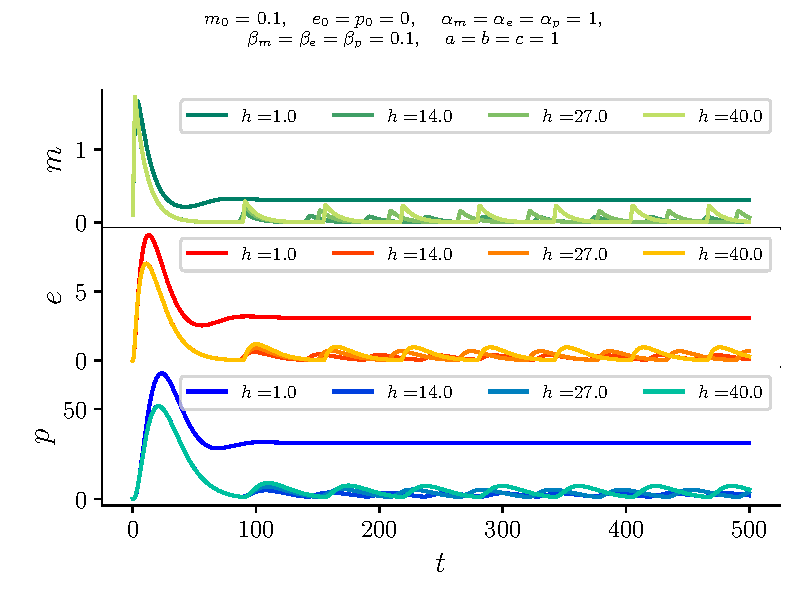
\includegraphics[width = 0.999\textwidth]{figuras/ex01-concentracion-h.pdf}
  \end{subfigure}\quad
  \caption{Resolución numérica de las Ecs. \ref{eq:ecuaciones}. para distintos valores de $h$.}
  \label{fig:figuras/ex01-concentracion-h}
\end{figure*}

En la Fig. \ref{fig:figuras/ex01-concentracion-h} se tiene la solución numérica de las Ecs. \ref{eq:ecuaciones}. para distintos valores de $h$.

%**********
\begin{figure*}[ht!]
  \centering
  \begin{subfigure}[b]{0.49\linewidth}
      \centering
      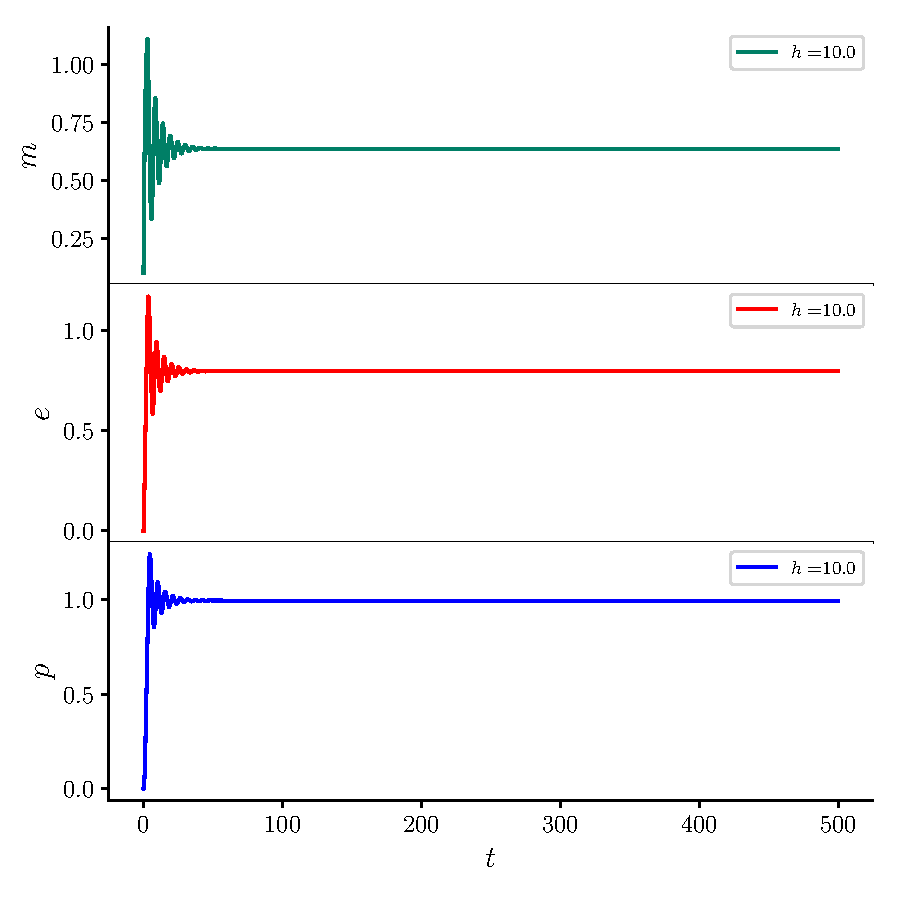
\includegraphics[width = 0.999\textwidth]{figuras/ex01-concentracion-h-osc-kill.pdf}
      \label{fig:figuras/ex01-concentracion-h-osc-kill}
  \end{subfigure}
  \begin{subfigure}[b]{0.49\linewidth}
      \centering
      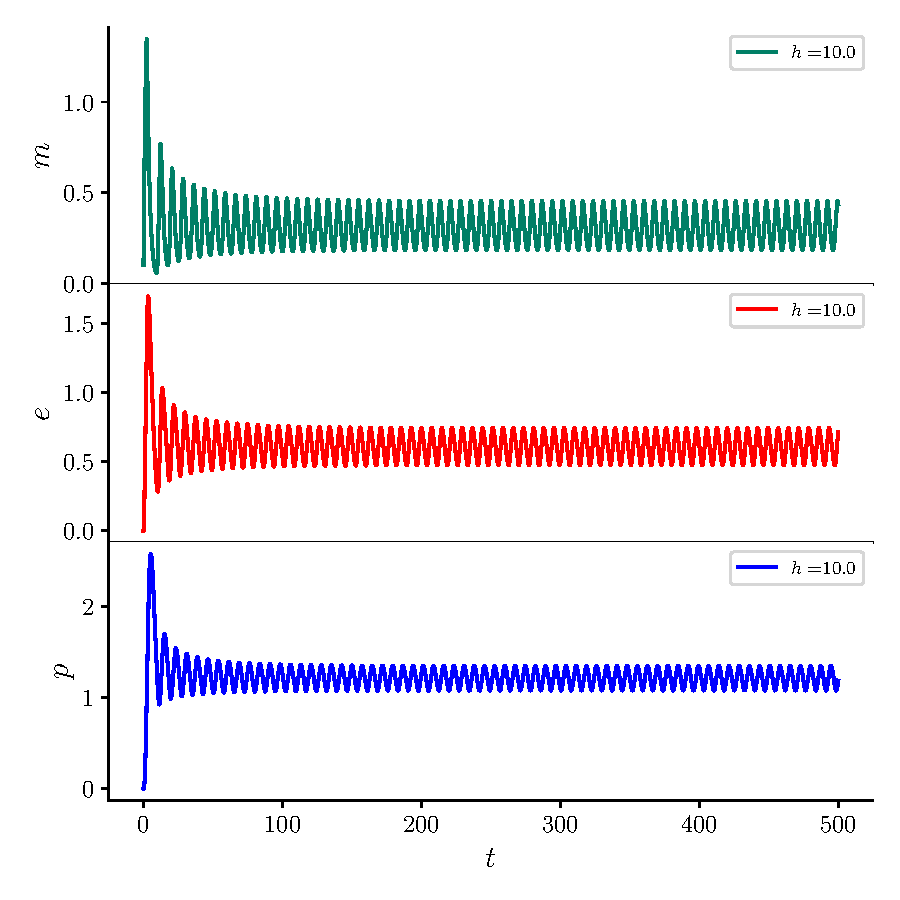
\includegraphics[width = 0.999\textwidth]{figuras/ex01-concentracion-h-osc.pdf}
      \label{fig:figuras/ex01-concentracion-h-osc}
  \end{subfigure}\quad
  \caption{Comparación entre dos sistemas con el mismo exponente de Hill, pero a diferentes valores de las degradaciones $\beta$.}
  \label{fig:figuras/ex01-concentracion-osc}
\end{figure*}
%**********

Por otro lado, en la Fig. \ref{fig:figuras/ex01-concentracion-osc}. se tiene una comparación entre dos sistemas con el mismo exponente de Hill, pero a diferentes valores de las degradaciones $\beta$.

% ███████╗██╗  ██╗    ██████╗  
% ██╔════╝╚██╗██╔╝    ╚════██╗
% █████╗   ╚███╔╝      █████╔╝
% ██╔══╝   ██╔██╗     ██╔═══╝ 
% ███████╗██╔╝ ██╗    ███████╗
% ╚══════╝╚═╝  ╚═╝    ╚══════╝

\section{Resolución Ej. 2}

%%%%%%%%%%%%%%%%%%%%%%%%%%%%%%%%%%%%%%%%%%%%%%%%%%%%%%%%%%%%%%%%%%%%%%
% \sepline
%%%%%%%%%%%%%%%%%%%%%%%%%%%%%%%%%%%%%%%%%%%%%%%%%%%%%%%%%%%%%%%%%%%%%%

Se estudia la dinámica del sistema de dos genes con represión mutua dada por:
$$\left\lbrace
\begin{aligned}
\frac{d m_{1}}{dt} &= \alpha_{m} g_{R}(p 2)-\beta_{m} m_{1} \\
\frac{d m_{2}}{dt} &= \alpha_{m} g_{R}(p 1)-\beta_{m} m_{2} \\
\frac{d p_{1}}{dt} &= \alpha_{p} m_{1}-\beta_{p} p_{1} \\
\frac{d p_{2}}{dt} &= \alpha_{p} m_{2}-\beta_{p} p_{2}
\end{aligned}\right.
$$

con tasas y funciones de represión iguales para ambos genes.
Reducción del sistema a dos variables
si $\beta_{m}>>\beta_{p}$, entonces la dinámica está dominada por la proteína, dado que la degradación del mRNA sucede muy rápidamente. Por ello, podemos suponer que $\frac{dm_1}{dt} \approx \frac{dm_2}{dt} \approx 0 .$ Con esto en cuneta el sistema de ecuaciones resulta:
$$\left\lbrace
\begin{aligned}
  m_{1} &=\frac{\alpha_{m}}{\beta_{m}} g_{R}\left(p_{2}\right) \\
  m_{2} &=\frac{\alpha_{m}}{\beta_{m}} g_{R}\left(p_{1}\right) \\
  \frac{dp_{1}}{dt} &= \alpha_{p} m_{1}-\beta_{p} p_{1} \\
  \frac{dp_{2}}{dt} &= \alpha_{p} m_{2}-\beta_{p} p_{2}
\end{aligned}\right.
\Rightarrow
\left\lbrace
\begin{aligned}
  m_{1} &=\frac{\alpha_{m}}{\beta_{m}} g_{R}\left(p_{2}\right) \\
  m_{2} &=\frac{\alpha_{m}}{\beta_{m}} g_{R}\left(p_{1}\right) \\
  \frac{dp_{1}}{dt} &=\alpha_{p} \frac{\alpha_{m}}{\beta_{m}} g_{R}\left(p_{2}\right)-\beta_{p} p_{1} \\
  \frac{dp_{2}}{dt} &=\alpha_{p} \frac{\alpha_{m}}{\beta_{m}} g_{R}\left(p_{1}\right)-\beta_{p} p_{2}
\end{aligned}\right.
$$

\begin{figure*}[ht!]
  \centering
  \begin{subfigure}[b]{0.49\linewidth}
    \centering
    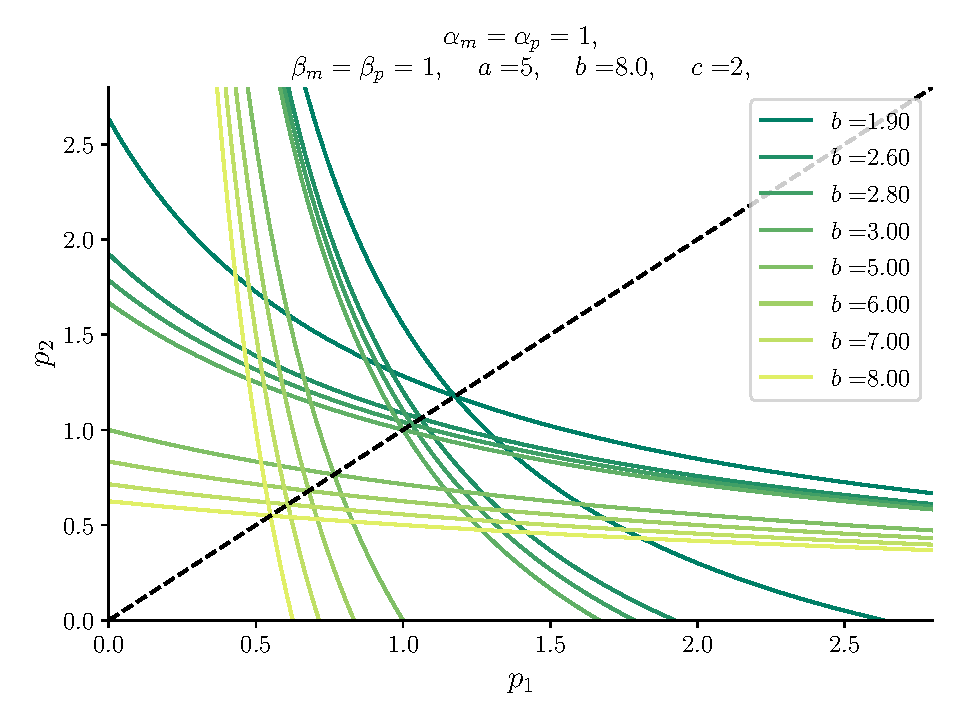
\includegraphics[width = 0.999\textwidth]{figuras/ex02-cosa1-3.pdf}
    \caption{}
    \label{fig:figuras/ex02-cosa1-3}
\end{subfigure}\quad
  \begin{subfigure}[b]{0.49\linewidth}
      \centering
      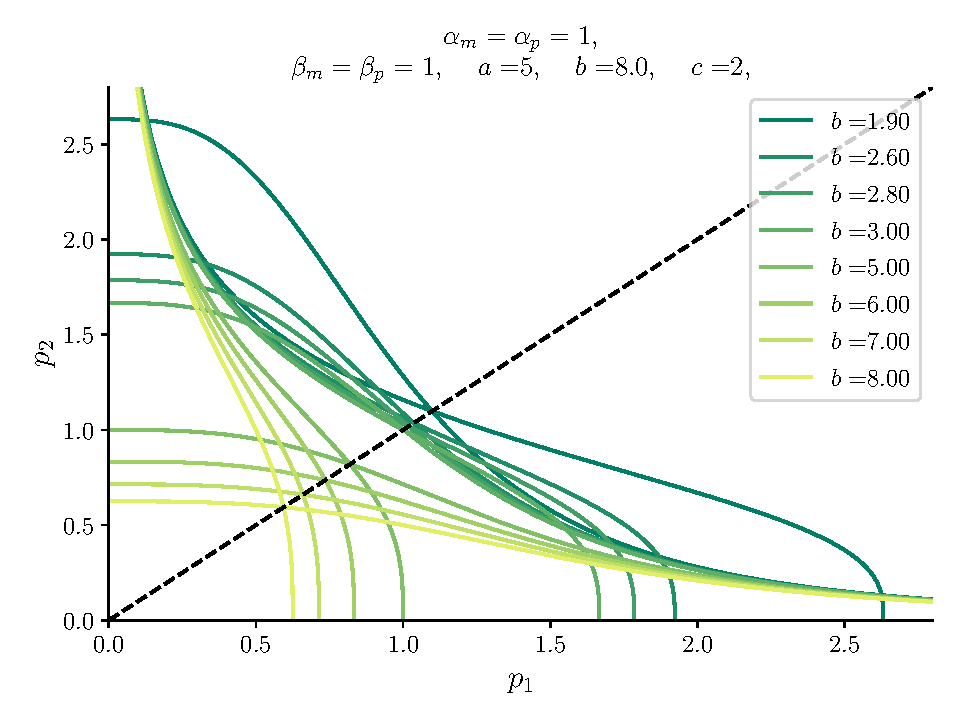
\includegraphics[width = 0.999\textwidth]{figuras/ex02-cosa1-2.pdf}
      \caption{}
      \label{fig:figuras/ex02-cosa1-2}
  \end{subfigure}\quad
  \caption{Puntos fijos del sistema para distintos valores del parámetro b.}
  \label{fig:figuras/ex02-puntos fijos}
\end{figure*}

Un análisis de estabilidad numérico de este sistema de ecuaciones reducido puede verse en la Fig. \ref{fig:figuras/ex02-puntos fijos}. Las intersecciones de curvas de un mismo color son los puntos fijos del sistema de ecuaciones.


\begin{figure*}[ht!]
  \centering
  \begin{subfigure}[b]{0.49\linewidth}
      \centering
      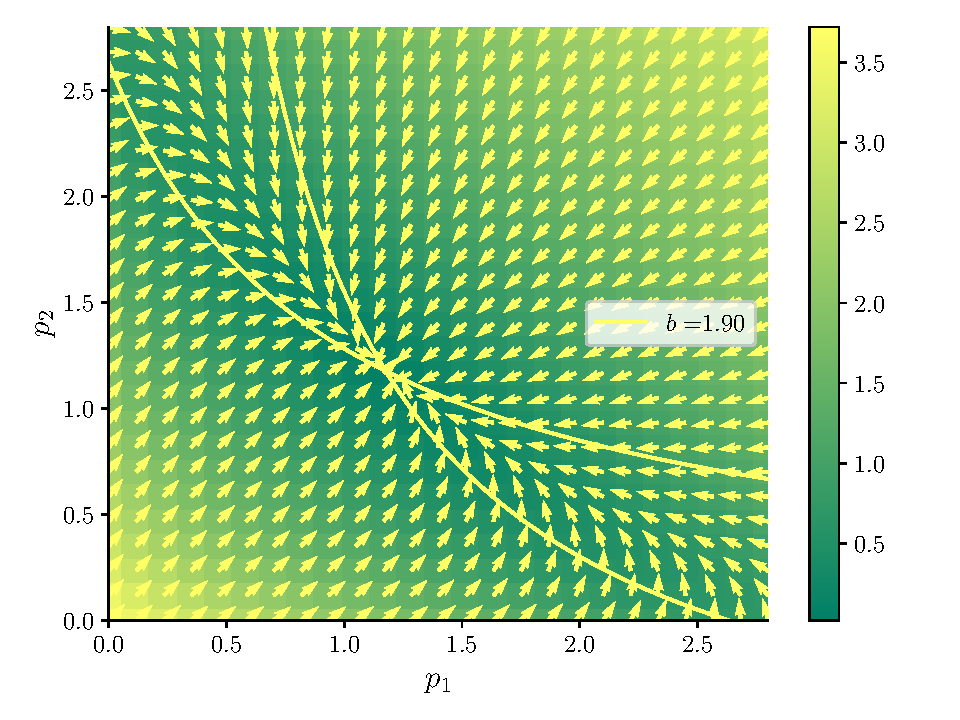
\includegraphics[width = 0.999\textwidth]{figuras/ex02-cosa3-0.pdf}
  \end{subfigure}\quad
  \begin{subfigure}[b]{0.49\linewidth}
      \centering
      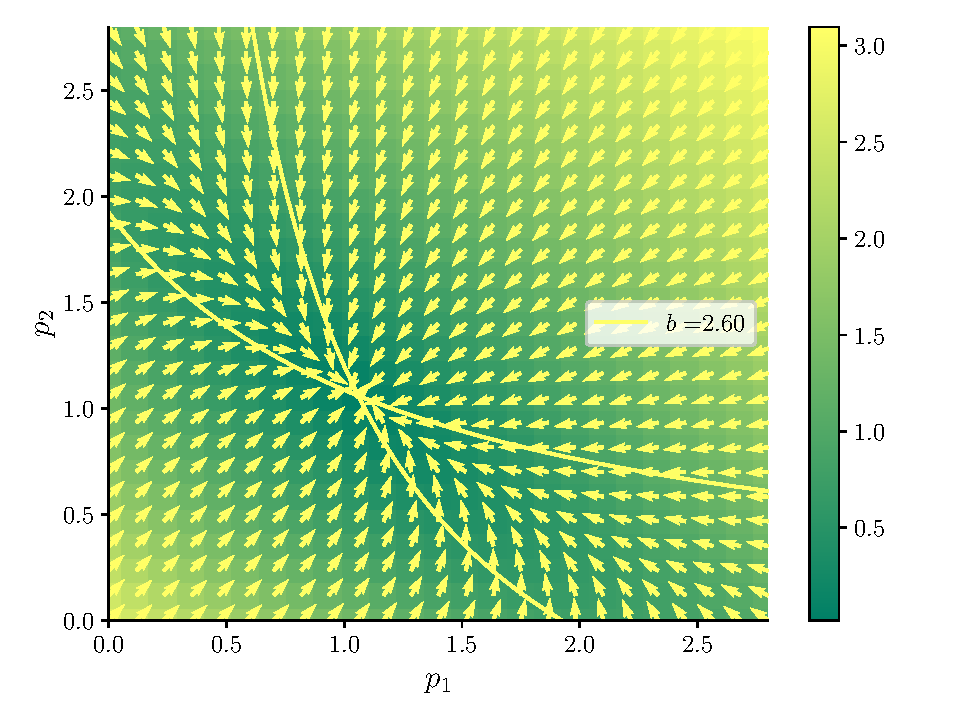
\includegraphics[width = 0.999\textwidth]{figuras/ex02-cosa3-1.pdf}
  \end{subfigure}\quad
  \begin{subfigure}[b]{0.49\linewidth}
      \centering
      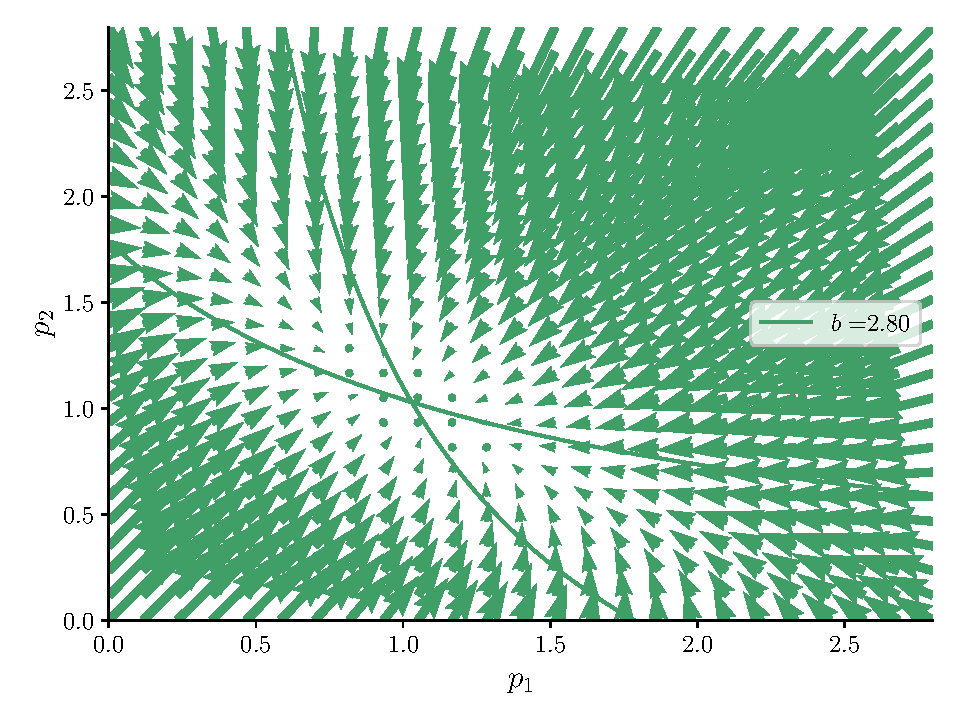
\includegraphics[width = 0.999\textwidth]{figuras/ex02-cosa3-2.pdf}
  \end{subfigure}\quad
  \begin{subfigure}[b]{0.49\linewidth}
      \centering
      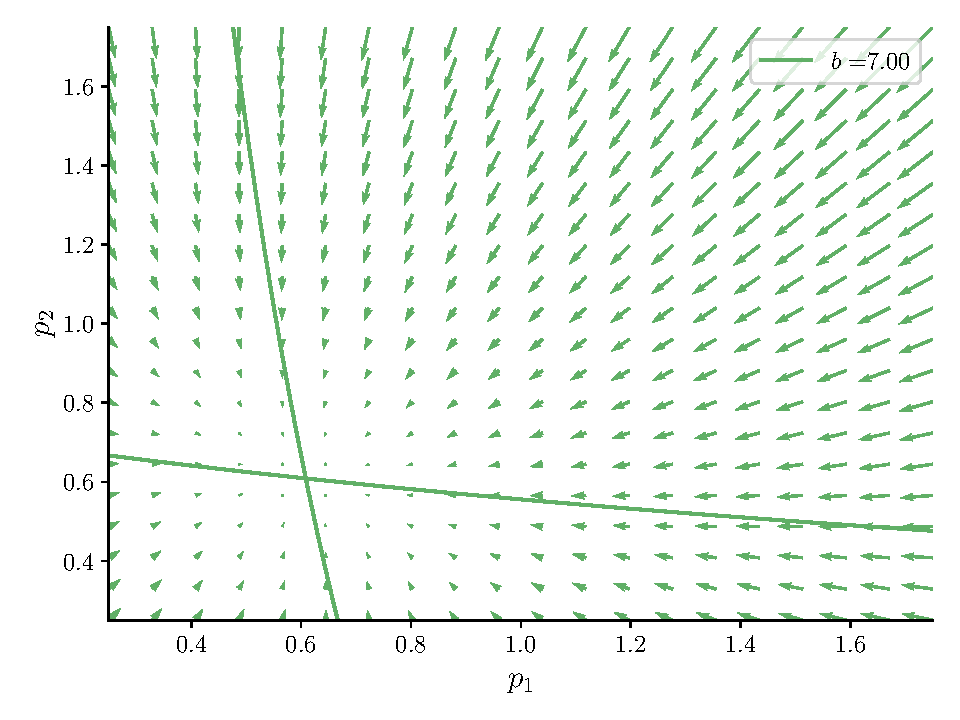
\includegraphics[width = 0.999\textwidth]{figuras/ex02-cosa3-3.pdf}
  \end{subfigure}\quad
  \begin{subfigure}[b]{0.49\linewidth}
      \centering
      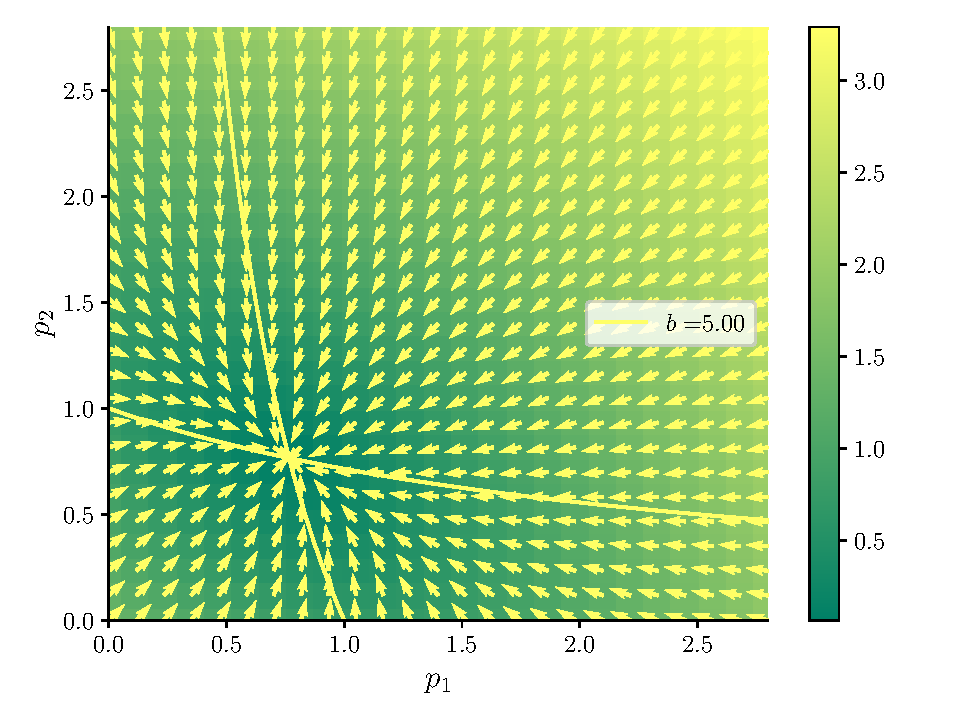
\includegraphics[width = 0.999\textwidth]{figuras/ex02-cosa3-4.pdf}
  \end{subfigure}\quad
  \begin{subfigure}[b]{0.49\linewidth}
      \centering
      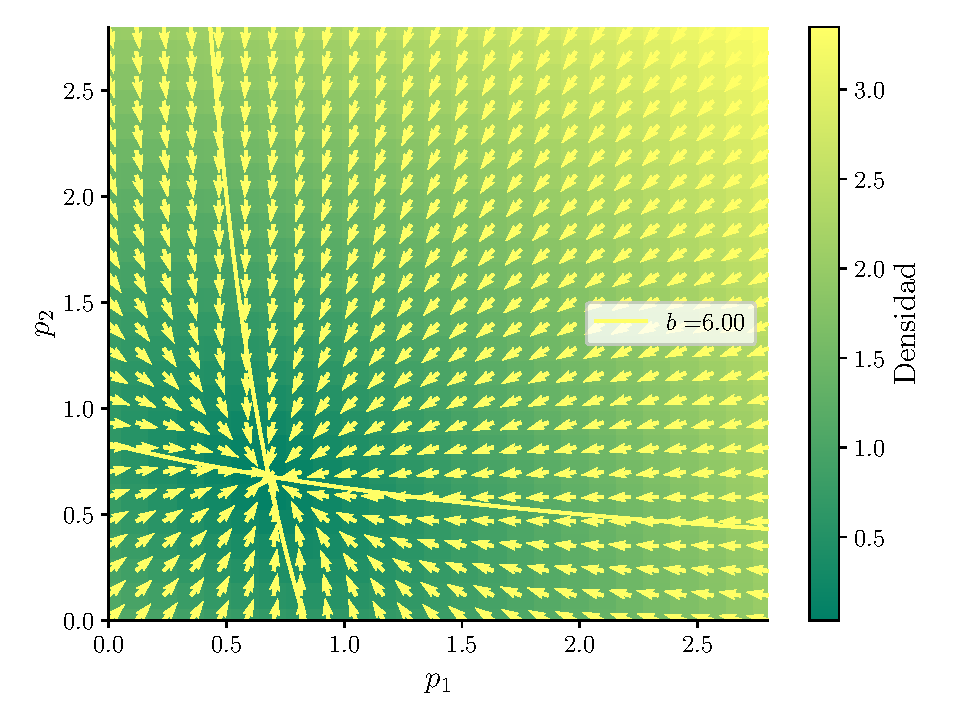
\includegraphics[width = 0.999\textwidth]{figuras/ex02-cosa3-5.pdf}
  \end{subfigure}\quad
  \begin{subfigure}[b]{0.49\linewidth}
      \centering
      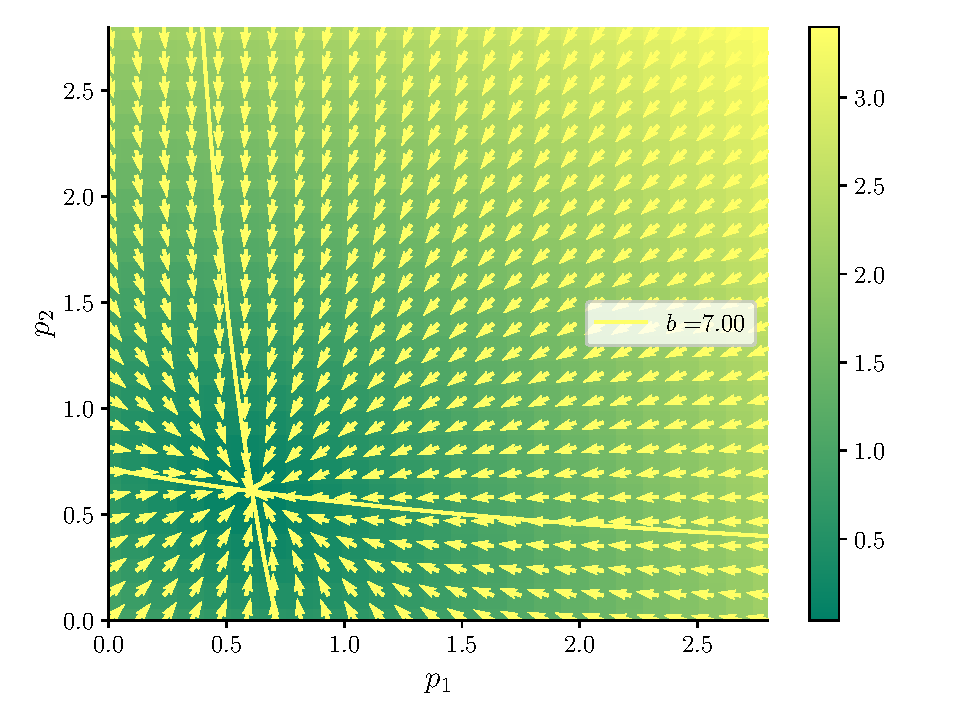
\includegraphics[width = 0.999\textwidth]{figuras/ex02-cosa3-6.pdf}
  \end{subfigure}\quad
  \begin{subfigure}[b]{0.49\linewidth}
      \centering
      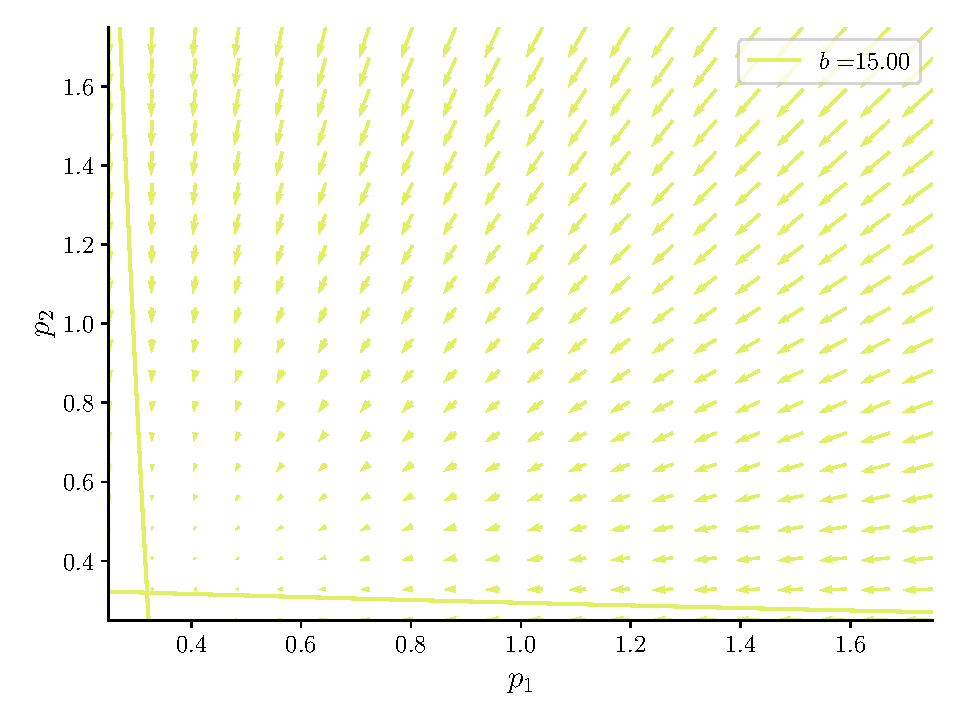
\includegraphics[width = 0.999\textwidth]{figuras/ex02-cosa3-7.pdf}
  \end{subfigure}\quad
  \caption{}
  \label{fig:figuras/ex02-cosa3}
\end{figure*}
%********** 

\begin{figure*}[ht!]
  \centering
  \begin{subfigure}[b]{0.49\linewidth}
      \centering
      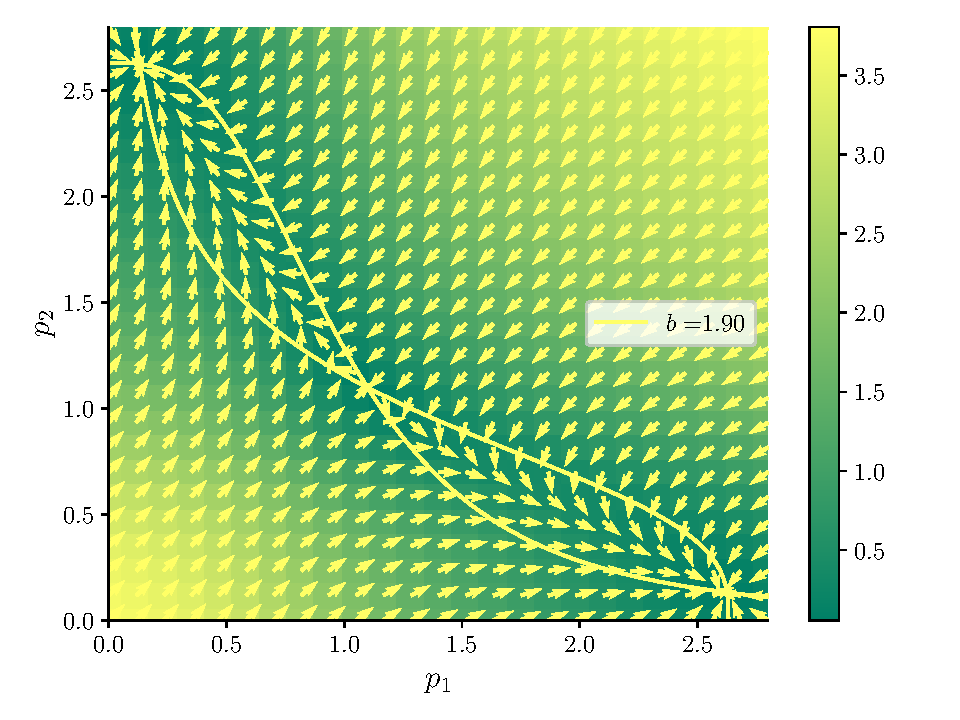
\includegraphics[width = 0.999\textwidth]{figuras/ex02-cosa2-0.pdf}
  \end{subfigure}\quad
  \begin{subfigure}[b]{0.49\linewidth}
      \centering
      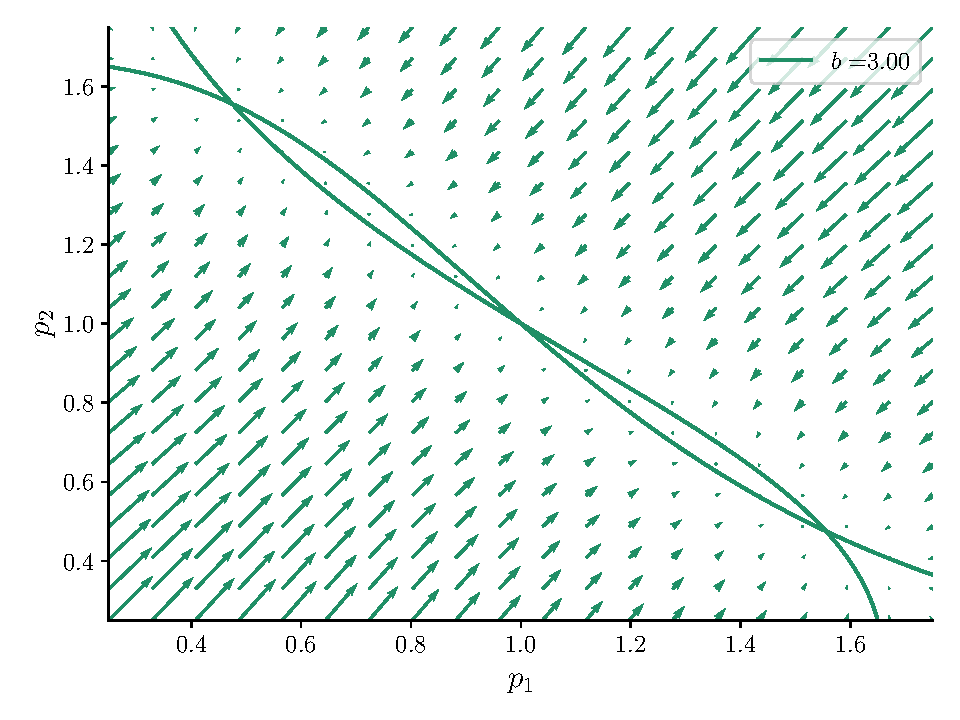
\includegraphics[width = 0.999\textwidth]{figuras/ex02-cosa2-1.pdf}
  \end{subfigure}\quad
  \begin{subfigure}[b]{0.49\linewidth}
      \centering
      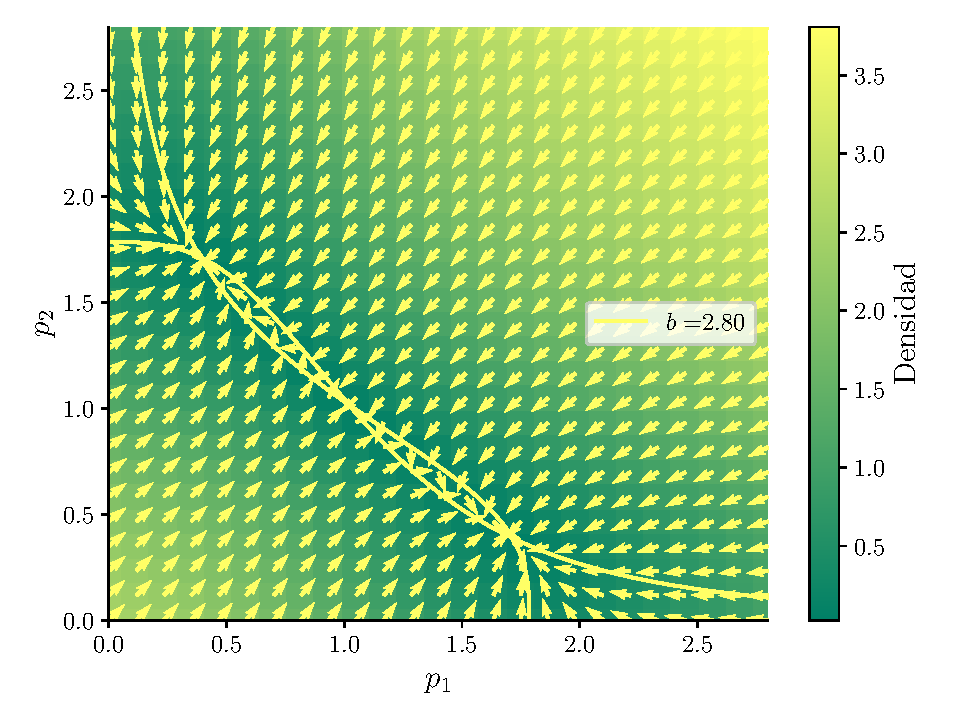
\includegraphics[width = 0.999\textwidth]{figuras/ex02-cosa2-2.pdf}
  \end{subfigure}\quad
  \begin{subfigure}[b]{0.49\linewidth}
      \centering
      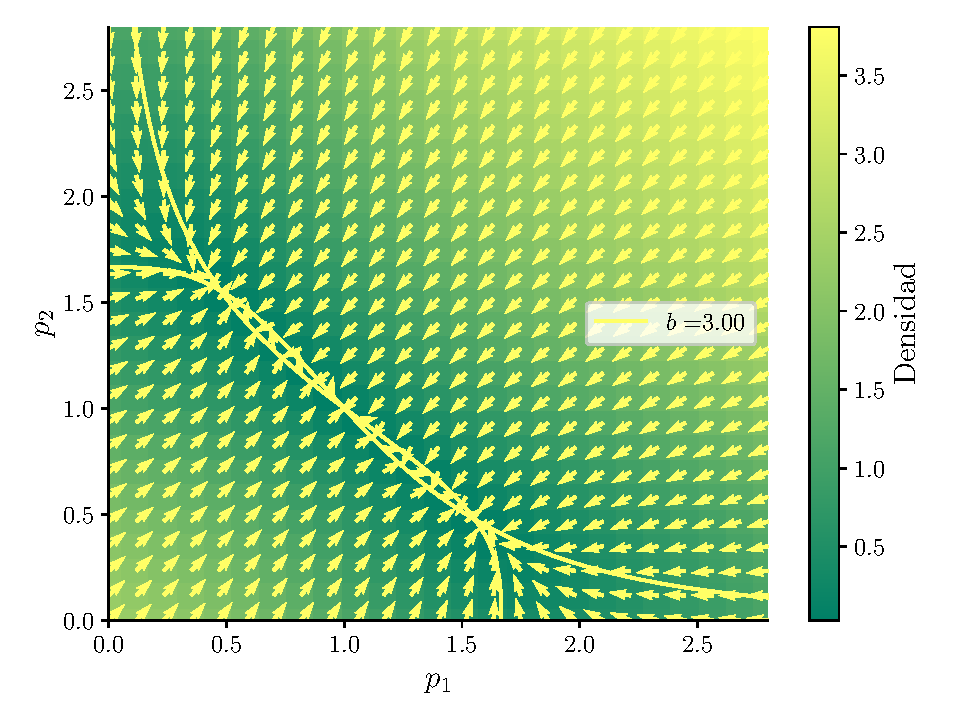
\includegraphics[width = 0.999\textwidth]{figuras/ex02-cosa2-3.pdf}
  \end{subfigure}\quad
  \begin{subfigure}[b]{0.49\linewidth}
      \centering
      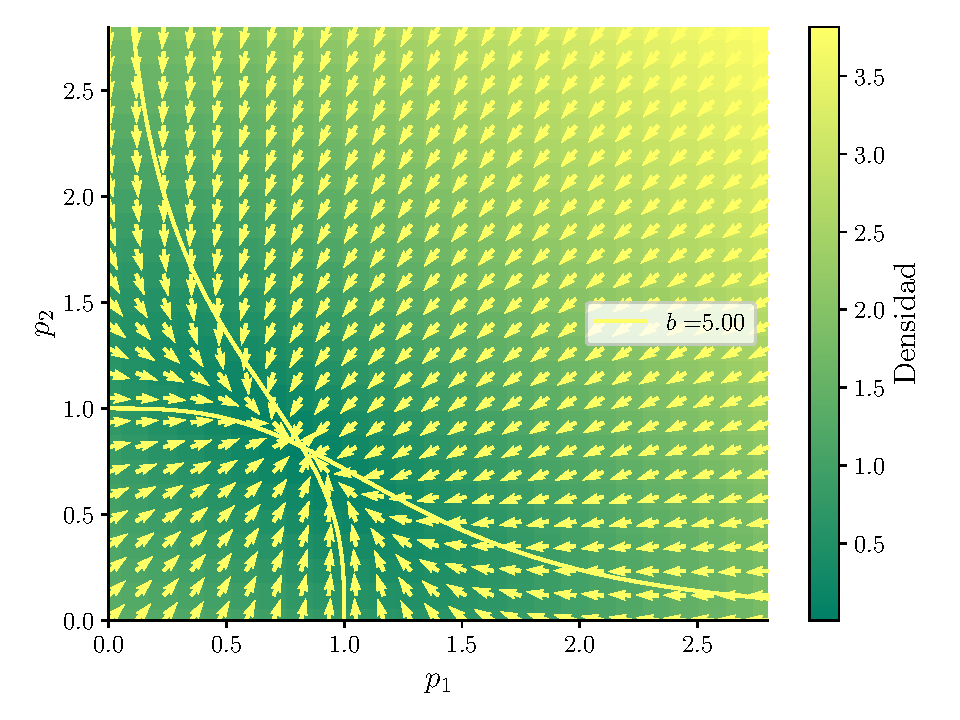
\includegraphics[width = 0.999\textwidth]{figuras/ex02-cosa2-4.pdf}
  \end{subfigure}\quad
  \begin{subfigure}[b]{0.49\linewidth}
      \centering
      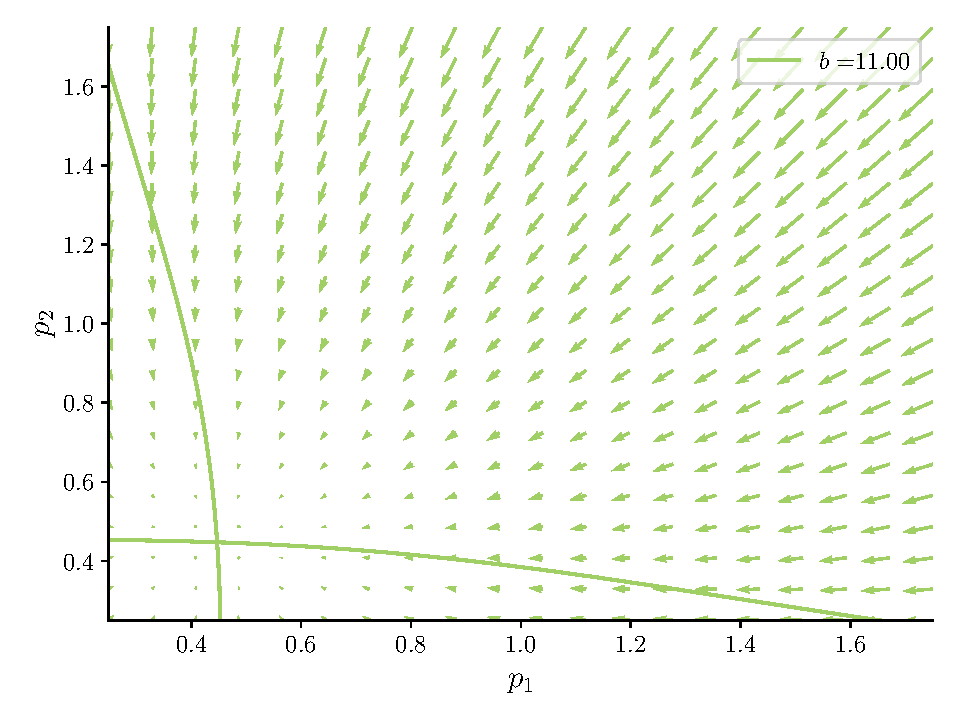
\includegraphics[width = 0.999\textwidth]{figuras/ex02-cosa2-5.pdf}
  \end{subfigure}\quad
  \begin{subfigure}[b]{0.49\linewidth}
      \centering
      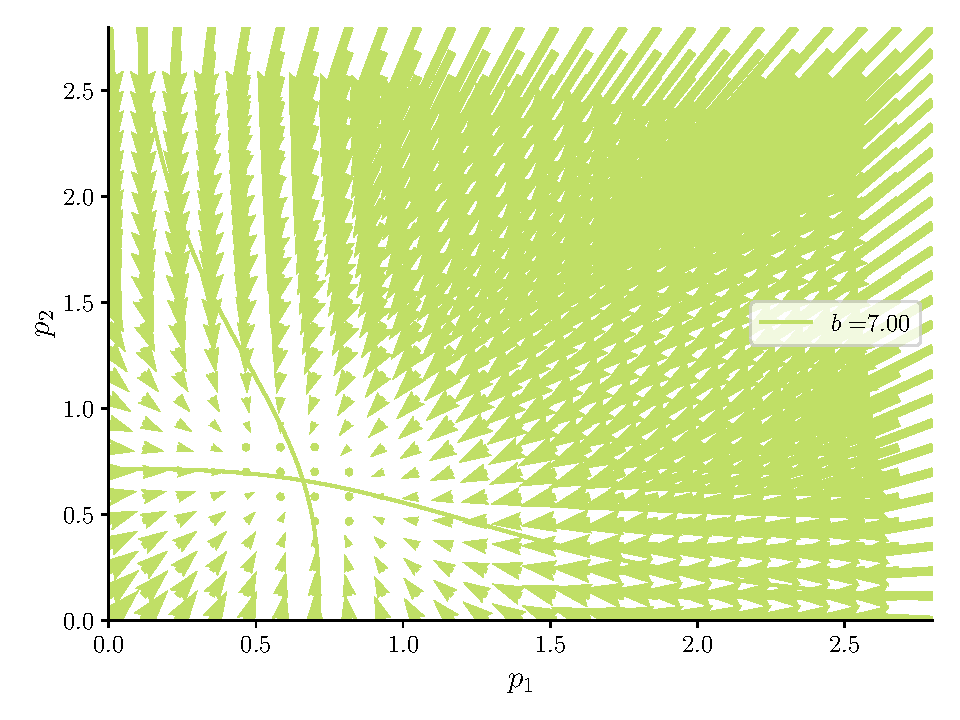
\includegraphics[width = 0.999\textwidth]{figuras/ex02-cosa2-6.pdf}
  \end{subfigure}\quad
  \begin{subfigure}[b]{0.49\linewidth}
      \centering
      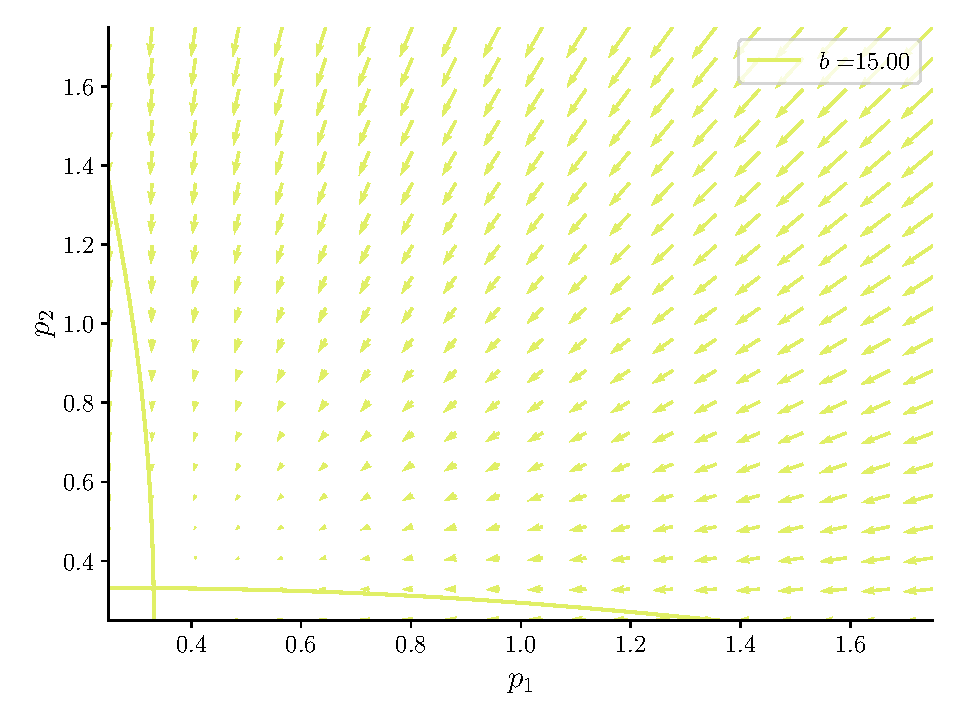
\includegraphics[width = 0.999\textwidth]{figuras/ex02-cosa2-7.pdf}
  \end{subfigure}\quad
  \caption{}
  \label{fig:figuras/ex02-cosa2}
\end{figure*}

En las Figs. \ref{fig:figuras/ex02-cosa3} y \ref{fig:figuras/ex02-cosa2} se tiene un gráfico del gradiente $(\frac{dp_1}{dt}, \frac{dp_2}{dt})$. 
Los gradientes de la Fig. \ref{fig:figuras/ex02-cosa3} corresponden a los parámetros de la Fig. \ref{fig:figuras/ex02-cosa1-3}.
Los gradientes de la Fig. \ref{fig:figuras/ex02-cosa2} corresponden a los parámetros de la Fig. \ref{fig:figuras/ex02-cosa1-2}. 

Los gradientes de la Fig. \ref{fig:figuras/ex02-cosa2} indican que hay una bifurcación al alternar el parámetro b. Esta desaparece para las condiciones iniciales de la Fig. \ref{fig:figuras/ex02-cosa1-2}. Donde pasamos de un nodo estable a dos nodos estables y un punto saddle.



% \bibliography{sample}

\end{document}
